\documentclass[a4paper,answers,12pt]{exam} % answers
\usepackage[T1]{fontenc}
\usepackage{amsmath}
\usepackage{amssymb}
\usepackage{enumerate}
\usepackage{bm}
\usepackage{advdate}
\usepackage{datetime}
\usepackage{hyperref}
\usepackage[mathcal]{eucal}
\usepackage{dsfont}
\usepackage[numbered,framed]{matlab-prettifier}
\usepackage{graphicx}
\usepackage[thehwcnt=0]{iidef}
\newcommand{\bx}{\bm{x}}    % x, vec
\newcommand{\bX}{\bm{X}}    % X, mat
\newcommand{\by}{\bm{y}}    % y, vec
\newcommand*{\defeq}{\stackrel{\text{def}}{=}}




\newcommand{\ut}{\underline{t}}    % t, vec

\newcommand{\bA}{\bm{A}}    % A, mat
\newcommand{\bn}{\bm{n}}    % n, mat

\newcommand{\bc}{\bm{c}}    % c, vec
\newcommand{\bu}{\bm{u}}    % u, vec
\newcommand{\bv}{\bm{v}}    % v, vec
\newcommand{\bw}{\bm{w}}    % w, vec
\newcommand{\bT}{\bm{T}}    % T, mat
\newcommand{\bW}{\bm{W}}

\newcommand{\bY}{\bm{Y}}     % y, vec
\newcommand{\rvby}{\bm{\mathsf{y}}}    % y, rv. vec
\newcommand{\rvbx}{\bm{\mathsf{x}}}    % x, rv. vec
\newcommand{\bz}{\bm{z}} 
%\newcommand{\bx}{\bm{x}}% z, vec
% \newcommand{\bm}{\bm{m}}    % m, vec
\newcommand{\bt}{\bm{t}}    % t, vec
\newcommand{\bzero}{\bm{0}}    % 0, vec

\newcommand{\balpha}{\bm{\alpha}}    % alpha, vec
\newcommand{\bxi}{\bm{\xi}}    % xi, vec
\newcommand{\btheta}{\bm{\theta}}
\newcommand{\bTheta}{\bm{\Theta}}    % theta, vec
\newcommand{\bmu}{\bm{\mu}}    % mu, vec

\newcommand{\bSigma}{\bm{\Sigma}}    % Sigma, vec

\newcommand{\cL}{\mathcal{L}}  
\newcommand{\cX}{\mathcal{X}}  



\newcommand{\rvv}{\mathsf{v}}    % v, r.v.
\newcommand{\rvm}{\mathsf{m}}    % m, r.v.
\newcommand{\rvt}{\mathsf{t}}    % t, r.v.

\newcommand{\urvt}{\underline{\mathsf{t}}}    % t, r.v. vec

\newcommand{\T}{\mathrm{T}}    % transpose
\newcommand{\F}{\mathrm{F}}    % Frobenius
\newcommand{\BLS}{\mathrm{BLS}}    % BLS
\newcommand{\LLS}{\mathrm{LLS}}    % LLS
\newcommand{\MVU}{\mathrm{MVU}}    % MVU

\DeclareMathOperator*{\maximize}{maximize}    % maximize
\DeclareMathOperator*{\minimize}{minimize}    % minimize
\newcommand{\st}{\mathrm{subject~to}}    % minimize
\DeclareMathOperator{\tr}{Tr}
% \newcommand{\E}[1]{\mathbb{E}\left[{#1}\right]}
% \newcommand{\Prob}[1]{\mathbb{P}\left({#1}\right)}


\usepackage{url}
\DeclareMathOperator{\norm}{Norm}
\DeclareMathOperator{\invgamma}{NormInvGam}
\newcommand{\talpha}{\tilde{\alpha}}
\newcommand{\tbeta}{\tilde{\beta}}
\newcommand{\tgamma}{\tilde{\gamma}}
\newcommand{\tdelta}{\tilde{\delta}}

\usepackage{color}

\def\changemargin#1#2{\list{}{\rightmargin#2\leftmargin#1}\item[]}
\let\endchangemargin=\endlist 
 
\newcommand{\yang}[1]{{\sf\color{blue}Yang: #1}}  

\begin{document}
\pagestyle{headandfoot}
\runningheadrule
\firstpageheader{Learning from Data}{Midterm Exam}{November 6, 2020}
\runningheader{Learning from Data}
              {Midterm Exam, Page \thepage\ of \numpages}
              {November 6, 2020}
\firstpagefooter{}{}{}
\runningfooter{}{}{}
%\topskip0pt
\vspace*{\fill}
\centering
Time Limit: 150 Minutes\\
\qquad\\
8:50 - 11:20\\
\qquad\\
Total score: 100+10 credit
\vspace{0.5em}

\begin{center}
  \fbox{\fbox{\parbox{6.5in}{%\centering
        \begin{itemize}
        \item Answer the questions in the spaces provided on the
          \textbf{answer sheets}.  If you run out of room for an answer,
          continue on the back of the page.

        \item \textbf{If you use a ``fundamental theorem'' you must indicate this} and explain
          why the theorem may be applied.

        \item \textbf{Organize your work}, in a reasonably neat and coherent way, in
          the space provided. Work scattered all over the page without a clear ordering will 
          receive very little credit.  

        \item \textbf{Mysterious or unsupported answers will not receive full
            credit}.  A correct answer, unsupported by calculations, explanation,
          or algebraic work will receive no credit; an incorrect answer supported
          by substantially correct calculations and explanations might still receive
          partial credit.
        \end{itemize}
}}}
\end{center}

\vspace{0.5in}
\centering
\begin{minipage}{0.5\textwidth}
  \makebox[\textwidth]{Name:\enspace\hrulefill}

  \vspace{2em}
  \makebox[\textwidth]{Student Number:\enspace\hrulefill} \\ 
\end{minipage}

\vspace*{\fill}
\hrulefill \\
\vspace{1em}
\textbf{Possibly useful facts:}
\begin{enumerate}

	
	%\item The PDF of $\rvbx \sim \mathcal{N}(\bmu, \bSigma)$:
	%\begin{equation*}
	%p_{\rvbx}(\bx) = \frac{1}{(2\pi)^{\frac{n}{2}}|\bSigma|^{\frac{1}{2}}} %\exp{\left(-\frac{1}{2}(\bx - \bmu)^\T \bSigma^{-1} (\bx - \bmu)\right)}.
	%\end{equation*} 
	
	\item For compatible size matrices and vectors, we have 
	\begin{align*}
	    \dfrac{\partial \bm{a}^{\T}\bx}{\partial \bx} = \bm{a},\qquad
	   \dfrac{\partial \bm{b^{\T}}\bX^{\T}\bm{D}\bX\bm{c}}{\partial \bX} = \bm{D}\bX\bm{b}\bm{c^{\T}} + \bm{D}\bX\bm{c}\bm{b^{\T}},\qquad
	   (\dfrac{\partial \ell}{\partial \bA})_{ij} = \dfrac{\partial \ell}{\partial \bA_{ij}}
	\end{align*}
	
	\item A class of distribution is in the exponential family if it can be written as
	\begin{equation*}
	    p(y;\bm{\eta}) = b(y)\exp(\bm{\eta}^{\T}T(y)-a(\bm{\eta}))
	\end{equation*}
\end{enumerate}
\newpage


\begin{questions}
	


	
  \question
 \begin{parts}
 \part(MLE \& Linear Regression) Consider the linear regression problem with Laplace measurement error: given $m$  samples $(\bx^{(1)}, y^{(1)}), \dots, (\bx^{(m)}, y^{(m)}), \bx^{(i)}\in\mathbb{R}^{n}, y\in\mathbb{R},i=1,\cdots,m$, we need to determine the parameters  $\bm{\theta}\in\mathbb{R}^{n}$  for the linear model: %The linear relationship between these variables can be written as
 \begin{align*}
     y^{(i)} = \btheta^{\top}\bx^{(i)} + v^{(i)},
 \end{align*}
 $v^{(i)}\in\mathbb{R}$ are i.i.d. Laplacian random variables with density function: 
 \[
 f(v) = \frac{1}{2\tau}e^{\frac{-|v-\mu|}{\tau}}
 \]where $\tau>0$ and $\mu$ is the mean value. 
 \begin{subparts}
 \subpart[5] %If we are going to use maximum likelihood estimation to estimate $\bm{\theta}$,
 Write down the log-likelihood function of this problem. 
 \subpart[5] For data $((1,1)^{\top},1), ((1,2)^{\top},-1)$ and $\tau=1, \mu=0$, derive the maximum likelihood estimator of $\bm{\theta}$.
 \end{subparts}
 \begin{solution}
 \begin{enumerate}[label=\roman*]
 \item Define $f(\bx, y) = \frac{1}{2\tau}e^{\frac{-|y-\btheta^{\top}\bx-\mu|}{\tau}}$.
 

 The log likelihood function can be
 written as
 \begin{align*}
\log \ell(\bx, y) &= \log \prod_{i=1}^m f(\bx^{(i)}, y^{(i)}) \\     
& = \sum_{i=1}^m \log f(\bx^{(i)}, y^{(i)}) ....2) \\
& = \sum_{i=1}^m \left(-\frac{|y^{(i)}-\btheta^{\top}\bx^{(i)}-\mu|}{\tau} - \log (2\tau) \right)\\
& = - m \log (2\tau) -\frac{1}{\tau}\sum_{i=1}^m
|y^{(i)} - \btheta^{\top}\bx^{(i)}- \mu| \score{5}
 \end{align*}
 \item The maximum likelihood estimator of 
 $\btheta$ is the optimal solution to the
 following optimization problem:
\begin{align*}
 \min_{\theta_1, \theta_2} | \theta_1 + \theta_2 - 1 |
 + | \theta_1 + 2\theta_2 + 1 | \score{3}
\end{align*}
 \end{enumerate}
 in which we let
 \begin{align*}
     \theta_1 + \theta_2 - 1 & = 0 \\
     \theta_1 + 2\theta_2 + 1 & = 0 \score{4}
 \end{align*}
 and we have $\btheta = (3, -2)$ \score{5}
 \end{solution}
 \part[15](Least Square)
 Given data  $(\bx^{(1)}, \by^{(1)}), \dots, (\bx^{(m)}, \by^{(m)})$, where $\bx^{(i)} \in \mathbb{R}^n$ represents the input features, and $\by^{(i)} \in \mathbb{R}^l$ is the output (label). 
  
  Suppose we apply a weight $w_j$ to the $jth$ feature of each input sample, (i.e. when features have different importance), we could extend the least square problem as follows:  
  \[
  \minimize_{\bTheta}\frac{1}{2} \sum_{i=1}^m\sum_{j=1}^{l}{w_j} \left((\bTheta^\T \bx^{(i)})_{j}- \by^{(i)}_{j}\right)^2
  \]
  where $w_j>0$ for $j=1,\dots,n$, and  $\bTheta \in \mathbb{R}^{n\times l}$ is the parameter matrix.
  
%  Let's write the positive weights $\{w_j\}$ as the entries of diagonal matrix $\bm{W}$, which means you can write $\bm{W}$ as $\bm{W}=\mathbf{diag} (w_1,w_2,\dots, w_l)$.\\
  Please derive the closed form solution for the optimal $\bTheta$ in matrix form.
  
  Hint: you can  denote the design matrix by $\bX \defeq [\bx^{(1)}, \dots, \bx^{(m)}]^{\T}$,   let $\bY \defeq [\by^{(1)}, \cdots, \by^{(m)}]^{\T}$, and let    $\bW=\mathbf{diag} (w_1,w_2,\dots, w_l)$.\\
  (You will get deduction if you write down your solution with summation notations)
\end{parts}
\begin{solution}
The loss function be written down as 
\begin{align*}
J(\bTheta) &= \frac{1}{2} \sum_{j=1}^{l} \sum_{i=1}^{m} \bW_{jj}(\bX\bTheta-\bY)^2_{ij} \\
&= \frac12 \tr\left((\bX\bTheta-\bY)^\T(\bX\bTheta-\bY)\bW\right) \score{8}
\end{align*}
% if the Trace operation is forgotten, losing one point
Then do the derivative
\begin{align*}
\nabla_{\bTheta}J(\bTheta)&=\frac12 \nabla_{\bTheta}\left[\tr\left(\bTheta^\T\bX^\T\bX\bTheta\bW\right)-\tr\left(\bTheta^\T\bX^\T\bY\bW\right)-\tr\left(\bY^\T\bX\bTheta\bW\right)\right]\\
% see matrix cookbook,
% how to take derivatives about trace function
 &=\frac12 \left[2\bX^\T\bX\bTheta\bW-2\bX^\T\bY\bW\right]\\
&=(\bX^\T\bX\bTheta-\bX^\T\bY)\bW \score{13}
\end{align*}
Let $\nabla_{\bTheta}J(\bTheta) = 0$, the solution is
\begin{equation*}
\bTheta=\left(\bX^\T\bX\right)^{-1}\bX^\T\bY \score{15}
\end{equation*}
% some students get the result $\bTheta=\left(\bw\bX^\T\bX\right)^{-1}\bw\bX^\T\bY \score{15}$
% The extra $\bW$ can be cancelled out. In such case, he will lose one point.
% For component-wise solution, if the students can write down the derivatives, points 5
% simplification, point 10
% write in compact matrix form, point 15
\end{solution}

  \question(SVM)
  We are given a training dataset of $m$ points of the form $(\bx^{(1)}, y^{(1)}), \dots, (\bx^{(m)}, y^{(m)})$, where  $\bx^{(i)} \in \mathbb{R}^n$, $y^{(i)} \in \{-1, 1\}$, $(i = 1, \cdots, m)$. Suppose the data are linearly separable, and let $\bw^{\star\T}\bx + b^\star = 0$ denote the optimal separating hyperplane in SVM.
  
\begin{parts}
  \begin{part}
  Consider the case $n = 2$. Evaluate $(\bw^{\star}, b^{\star})$ and list the support vectors for the following cases:
  \begin{subparts}
    \subpart[10] $m = 2$ with $y^{(1)} = 1, y^{(2)} = -1$ and $\bx^{(i)} = (y^{(i)}, y^{(i)})^{\T}, i = 1, 2$.
    \subpart[10] $m = 3$ with $y^{(1)} = 1, y^{(2)} = y^{(3)} = -1$, $\bx^{(1)} = (1, 1)^{\T}, \bx^{(2)} = (-1, -1)^{\T}, \bx^{(3)} = (t, -1)^{\T}$, where $t \in \mathbb{R}\setminus\{-1\}$ is a given parameter.\\
    Hint: Can you find the support vectors by inspection? 
  \end{subparts}
  \end{part}
  \begin{solution}
  \begin{enumerate}[label=\roman*]
      \item Solving the dual problem of SVM:
      \begin{align*}
          \max_{\alpha_1, \alpha_2}
          \,& \alpha_1 + \alpha_2 - \frac{1}{2}
          (2\alpha_1^2+2\alpha_2^2 + 4 \alpha_1 \alpha_2) \\
          s.t. \,& \alpha_1, \alpha_2 \geq 0, \alpha_1 - \alpha_2 = 0 \score{5}
      \end{align*}
      We get $\alpha_1 = \alpha_2 = \frac{1}{4}$. \score{7}
      The optimal $\bw^*,b^*$ are
      \begin{align*}
          \bw^* & = (\alpha_1 + \alpha_2)(1,1)^\T = (\frac{1}{2},\frac{1}{2})^\T \score{8}\\
        b^* & = -\frac{1}{2}(\bw^\T(-1,-1)^\T - \bw^\T(1,1)^\T) = 0          \score{9}
      \end{align*}
      The support vectors are $\bx^{(1)}$ and
      $\bx^{(2)}$. \score{10}
      % plotting 6 points
      % results 4 points
      \item Using geometric method, we could get
      \begin{enumerate}[label=(\arabic*)]
          \item When $t < -1$, the support vector is $\bx^{(1)}$
          and $\bx^{(2)}$, with $\bw^* = (\frac{1}{2}, \frac{1}{2})^\T$
          and $b^* = 0$. \score{3}
          \item When $ -1 < t < 1$, the support vector is $\bx^{(1)}$
          and $\bx^{(3)}$, with $\bw^* = (\frac{2-2t}{t^2-2t+5}, \frac{4}{t^2-2t+5})^\T$
          and $b^* = \frac{t^2-1}{t^2-2t+5}$. \score{7}
          \item When $ t \geq 1 $, the support vector is $\bx^{(1)}$, $\bx^{(2)}$
          and $\bx^{(3)}$, with $\bw^* = (0,1)^\T$
          and $b^* = 0 $. \score{10}
      \end{enumerate}
      % 3 categories, 5 points
      % results, 10 points
  \end{enumerate}
  \end{solution}
   \begin{changemargin}{-1cm}{0.5cm} 

 In Parts b) and c), we will explore the geometric interpretation of the optimal parameter $\bw^*$: the length of $\bw^*$ is determined by the minimum distance between the convex hulls of training samples separated by the hyperplane.   
 \end{changemargin}
  \part[5]  Prove that
  \begin{align*}
      ||\bw^*|| \geq \max_{(i,j):y^{(i)}\neq y^{(j)}} \frac{2}{||\bx^{(i)}-\bx^{(j)}||}.
  \end{align*}
  \begin{solution}
  For any $y^{(i)}=1, y^{(j)}=-1$, from
  the optimal margin interpretation of
  SVM, we have
  \begin{align*}
      (\bw^*)^\T \bx^{(i)} + b &\geq 1 \score{1}\\
      -((\bw^*)^\T \bx^{(j)} + b) & \geq 1\score{2}
  \end{align*}
  Summing up the above two equations we have
  \begin{equation*}
      (\bw^*)^\T (\bx^{(i)}-\bx^{(j)}) \geq 2 \score{3}
  \end{equation*}
  Similarly, when $y^{(i)}=-1, y^{(j)}=1$
  we have $-(\bw^*)^\T (\bx^{(i)}-\bx^{(j)}) \geq 2$.
  Therefore, for any  $y^{(i)} \neq y^{(j)}$,
    \begin{equation*}
      |(\bw^*)^\T (\bx^{(i)}-\bx^{(j)})| \geq 2
  \end{equation*}
  
  Using Cauchy's inequality we have
	\begin{align*}  
  ||\bw^*|| \cdot ||\bx^{(i)}-\bx^{(j)}|| \geq |(\bw^*)^\T (\bx^{(i)}-\bx^{(j)})| \geq 2\score{5}
  \end{align*}
  Therefore, 
    \begin{align*}
      ||\bw^*|| \geq \max_{(i,j):y^{(i)}\neq y^{(j)}} \frac{2}{||\bx^{(i)}-\bx^{(j)}||}.
  \end{align*}
  \end{solution}
  \part[10]  Now define $C_1, C_2$ as the convex hull of positive samples and negative samples, respectively:
  \begin{equation*}
    \begin{aligned}
      C_1 &= \left\{\sum_{i = 1}^m \theta_i \bx^{(i)}\colon\theta_i \geq 0, \theta_i(y^{(i)} - 1) = 0, i = 1,\dots, m,~\sum_{i = 1}^m \theta_i = 1 \right\},\\
      C_2 &= \left\{\sum_{i = 1}^m \theta_i \bx^{(i)}\colon\theta_i \geq 0, \theta_i(y^{(i)} + 1) = 0, i = 1,\dots, m,~ \sum_{i = 1}^m \theta_i = 1\right\}.
    \end{aligned}
  \end{equation*}
  We can explain the convex hull in a graphic way. It is the minimal convex set containing all samples.\\
\begin{figure}[h]
	\centering
	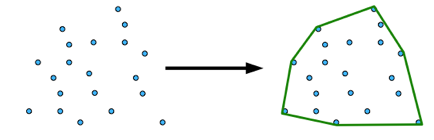
\includegraphics[width=8cm]{fig1.png}
%	\caption{Projection of $\by$ on column space of $\bX$}
	\label{fig1}
\end{figure}
  Prove that
  \begin{equation*}
    \|\bw^\star\| = \max_{\bu \in C_1, \bv \in C_2}\frac{2}{\|\bu - \bv\|}.
  \end{equation*}
\end{parts}
\begin{solution}
Suppose $\alpha_i, i = 1, \dots, m$ is the optimal solution to the dual problem of SVM.
Let $[m]_+ = \{1\leq i \leq m | \alpha_i > 0, y_i = 1 \}$ and $[m]_- = \{1\leq i \leq m | \alpha_i > 0, y_i = -1 \}$.
By the property of support vectors, we have
\begin{align}
          (\bw^*)^\T \bx^{(i)} + b &= 1 \,\forall i \in [m]_+ \label{eq:wxb}\\
      -((\bw^*)^\T \bx^{(j)} + b) &= 1 \,\forall j \in [m]_-\label{eq:wxb2}
\end{align}
Let $\alpha = \sum_{i \in [m]_+} \alpha_i$ and 
define
\begin{align*}
\theta_i =  \begin{cases} 
\alpha_i / \alpha & i \in [m]_+ \\
0 & i \not\in [m]_+
\end{cases}\quad \theta'_i =  \begin{cases} 
\alpha_i / \alpha & i \in [m]_- \\
0 & i \not\in [m]_-
\end{cases}
\end{align*}
Since $\sum_{i=1}^m \alpha_i y^{(i)} = 0$,
we also have $\alpha = \sum_{i\in [m]_-} \alpha_i$. Therefore,
$\sum_{i=1}^m \theta_i = \sum_{i=1}^m \theta'_i = 1$.
Let $\bu^* = \sum_{i=1}^m \theta_i \bx^{(i)}$
and $\bv^*= \sum_{i=1}^m \theta'_i \bx^{(i)}$.
From the definition of $C_1, C_2$, we have
$\bu^* \in C_1, \bv^* \in C_2$. Then from
(\ref{eq:wxb}, \ref{eq:wxb2}) we have
\begin{align*}
              (\bw^*)^\T \bu^* + b &= 1\\
      -((\bw^*)^\T \bv^* + b) &= 1  \score{3}
\end{align*}
That is
\begin{equation}\label{eq:bwuv}
    (\bw^*)^\T(\bu^* - \bv^*) = 2
\end{equation}
From the expression $\bw^* = \sum_{i=1}^m \alpha_i y^{(i)} \bx^{(i)}$ we have
\begin{equation}\label{eq:wuv}
    \frac{\bw^*}{\alpha} = \sum_{i \in [m]_+}
    \theta_i \bx^{(i)} - \sum_{i \in [m]_-}
    \theta'_i \bx^{(i)}
    = \bu^* - \bv ^* 
\end{equation}
From \eqref{eq:bwuv} and \eqref{eq:wuv} we have
$||\bw^*|| = \frac{2}{||\bu^* - \bv^*||}$. \score{5}
Similar to the proof of b), first we have
  \begin{align*}
      (\bw^*)^\T \bx^{(i)} + b &\geq 1, \textrm{ for } i \textrm{ satisfying } y^{(i)} = 1 \\
      -((\bw^*)^\T \bx^{(j)} + b) & \geq 1, \textrm{ for } i \textrm{ satisfying } y^{(i)} = -1 \score{7}
  \end{align*}
  Therefore,
    \begin{align*}
      (\bw^*)^\T \bu + b &\geq 1, \textrm{ for } \bu \in C_1\\
      -((\bw^*)^\T \bv + b) & \geq 1, \textrm{ for } \bv \in C_2  \score{9}
  \end{align*}
  Then by Cauchy's equality, 
  $|| \bw^* || \cdot ||\bu - \bv || \geq || (\bw^*)^\T (\bu - \bv)|| \geq 2$.\score{10}
  Thus we have shown that
    \begin{equation*}
    \|\bw^\star\| = \max_{\bu \in C_1, \bv \in C_2}\frac{2}{\|\bu - \bv\|}.
  \end{equation*}
\end{solution}
% \vspace{\footskip}
\question[20](Generative Model) We will explore the relationship between binary Naive Bayes classification and logistic regression.  %In class, we have learnt the relationship between GDA and Logistic Regression. %The connection between discriminative models and generative models goes on.
Given discrete random variables $(\bx, y)$ where %$\bx=(x_1,\cdots,x_n)^{\T}\in\mathbb{R}^{n}$ is an n-dimensional random vector,
$\bx=(x_1,\cdots,x_n)^{\T}$ is an n-dimensional binary random vector ($x_i\in\{0,1\}$)  and $y\in\{0,1\}$. By the Naive Bayes assumption,  we have %all elements in $\bx$ are conditional independent given $y$, i.e.,
\[
    P(\bx|y)=\prod_{i=1}^{n} P_{X_i|Y} (x_i|y), \forall \bx, y.
\]
%Let $\phi_y\defeq P_Y(y=1)$, and $\phi_{i|y=j}\defeq P_{X_i|Y} (x_i=1|y=j), i=1,\cdots,n, j=0,1$.
The class likelihood function $P_{Y|\bX}$   can be written in the form of logistic regression for some $\phi_y\defeq P_Y(y=1)$, and $\phi_{i|y=j}\defeq P_{X_i|Y} (x_i=1|y=j), i=1,\cdots,n, j=0,1$:
\begin{align*}
    P_{Y|\bX}(1|\bx) = \frac{1}{1+\exp{(-(\btheta^{\T}\bx+b))}}.
\end{align*}

Find $\btheta\in\mathbb{R}^n$ and $b\in\mathbb{R}$ in terms of $\phi_y$ and $\phi_{i|y=j},j=0,1$.

  
  \question[20] (Back Propagation) Consider the back propagation on the hidden-layer in a neural network. Given a batch of input feature $X=[x^{(1)}, x^{(2)}, \cdots, x^{(M)}]^T$ (Shape: $M\times D_0$), a set of weight \{$W\in\mathbb{R}^{D_0\times D_1}$, $b\in\mathbb{R}^{D_1\times 1}$\}, and element-wise Sigmoid activation function $\sigma(\cdot)$. The forward propagation on this hidden-layer is given by:
  \[
  F_1=XW+\1_Mb^T, \quad F_2=\sigma(F_1)
  \]
  where $\1_M$ is a vector composed of 1 in length $M$. $\sigma(\cdot)$ is element-wise Sigmoid function:
  \[
  [\sigma(X)]_{ij}=\frac{1}{1+\exp(-X_{ij})}
  \]
  Then in the back propagation stage, suppose we already know the gradients for some scalar loss function $l$ with respect to $F_2$ as $\nabla_{F_2}l$.
  \begin{parts}
  \part Proceed the back propagation and show that $\nabla_{F_1}l=(\nabla_{F_2}l)\odot F_2 \odot (1-F_2)$. where $(A\odot B)_{ij}=A_{ij}B_{ij}$ is element-wise production.
  \part Proceed the back propagation and evaluate $\nabla_{W}l$, $\nabla_{b}l$, and $\nabla_{X}l$.
  \end{parts}
\question (Extra Credit) Short Answers.
The following questions require a true/false accompanied by one sentence of explanation,
or a reasonably short answer (usually at most 1-2 sentences or a figure).
No credit will be given for answers without
a correct explanation.
\begin{parts}
\part[2] Let $f : \mathbb{R}^n \rightarrow \mathbb{R}$ be defined according to $f(x) = \frac{1}{2}\bx^{\T}\bA\bx + \bm{b}^{\T}\bx + c$, where
$\bA$ is symmetric positive definite. Suppose we use Newton’s method to minimize $f$.
Then Newton’s method will find the optimum in exactly one iteration. True/False? \\

\part[2] Logistic regression assumes $y|\bx$ is Bernoulli distributed, where $\bx$ is the data and $y$ is the label. Let's assume $p(y=1|\bx;\theta) = h_{\btheta}(\bx)$, in which $\btheta$ is the parameter we need to optimize and $h_{\btheta}(\bx)=\frac{1}{1+\exp\{-\btheta^{T}\bx^{(i)}\}}$. Given $m$ independent generated training examples, the log-likelihood function of such model is convex. True/False?%is $\ell(\btheta)=\sum\limits_{i=1}^{m} y^{(i)}\log(h_{\btheta}(\bx^{(i)})) + (1-y^{(i)})\log(1 - h_{\btheta}(\bx^{(i)}))$. And such log-likelihood function is convex. True/False? 
\part[2] In Softmax regression, $y|\bx$ is multinomial distributed with $p(y=i|\bx;\theta) = softmax(\btheta^{\T}\bx), i = 1,\cdots,k$, in which $softmax(z_i)\defeq \frac{\exp(z_i)}{\sum_{j=1}^k \exp(z_j)},i = 1,\cdots,k$. Then $p(y|\bx;\theta) = p(y|\bx;\psi-\theta)$. True/False? 
\part[2] Ordinary least square regression is equivalent to the maximum likelihood estimation of $\btheta$. True/False? 
\part[2] $Multinomial(\phi_1,\cdots,\phi_k)$ is in the exponential family. True/False? 



\end{parts}

\end{questions}
\end{document}
%%% Local Variables:
%%% mode: latex
%%% TeX-master: t
%%% End:

%  LocalWords:  headandfoot

